\documentclass[a4paper]{scrartcl}
\usepackage[utf8]{inputenc}
\usepackage{ngerman}
\usepackage{mathtools}
\usepackage{amssymb}
\usepackage{pdfpages}
\usepackage{mathtools}
\usepackage{listings}
\usepackage{tikz}
\usepackage{qtree}
\usepackage{hyperref}
\usetikzlibrary{arrows,automata}
\usetikzlibrary{shapes.multipart}
\usetikzlibrary{calc}

\title{Künstliche Intelligenz}
\date{SS 2015}
\author{Markus Klemm.net}

\lstdefinestyle{customc}{
  belowcaptionskip=1\baselineskip,
  breaklines=true,
  frame=L,
  xleftmargin=\parindent,
  language=C,
  showstringspaces=false,
  basicstyle=\footnotesize\ttfamily,
  keywordstyle=\bfseries\color{green!40!black},
  commentstyle=\itshape\color{purple!40!black},
  identifierstyle=\color{blue},
  stringstyle=\color{orange},
}

\begin{document}
\maketitle
\tableofcontents

%Inhalte
%Prädikatenlogik
%Prolog-Programmierung
%Logisches Schließen
%Computeralgebra
%Sprachverarbeitung
%Problemlösen durch Suche
%%A*-Suche
%Bayes'sche Netze

\section{Prädikatenlogik}
\subsection{Problem} Aussagenlogik ist wenig mächtig. Aussagen, die sich nicht formulieren lassen:
\begin{itemize}
\item Alle Vögel können fliegen.
\item Wenn X eine Katze ist, dann ist X ein Haustier.
\item Für jedes Land gibt es eine Hauptstadt.
\end{itemize}
In der Prädikatenlogik betrachten wir zunächst eine (unwichtige) Menge $U$ (Universum), die alle zu betrachtenden Objekte (Vögel, Katzen, Länder) enthält.
Davon betrachten wir Teilmengen, z.B. die Menge aller Vögel (also eine einstellige Relation) oder die Menge aller Verheirateten (also eine mehrstellige Relation).
\subsection{Definition}
Sei $V$ eine Menge von Variablen, $K$ eine Menge von Konstanten, $F$ eine Menge von Funktionssymbolen.
\begin{itemize}
\item Dann sind alle Variablen in $V$ und Konstanten in $K$, Terme.
\item Wenn $t_1,\dots,t_n$ Terme und $f$ ein $n$-stelliges Funktionssymbol sind, dann ist auch $f(t_1,\dots,t_n)$ ein Term.
\end{itemize}
\paragraph{Beispiel} $V=\{x,y,z\},K=\{a,b,c\},F=\{+,*\}$ Terme sind $x,y,a,x+a,(x+a)*y$.

\subsection{Definition} Sei eine Menge von Prädikatensymbolen gegeben. Die Formeln der Prädikatenlogik sind induktiv.

\begin{itemize}
\item Wenn $t_1,\dots,t_n$ Terme und $P$ ein Prädikatensymbol der Stelligkeit $n$ ist, dann ist $P(t_1,\dots,t_n)$ eine Formel.
\item Wenn $F,G$ Formeln sind, dann auch $F \wedge G, F\vee G, \neg F$.
\item Wenn $x$ eine Variable und $F$ eine Formel sind, dann auch $\forall x F$, sowie $\exists x F$.
\end{itemize}
\paragraph{Beispiel} 
\begin{itemize}
\item katze(reni)
\item $\forall x (\text{katze}(x) \rightarrow \text{haustier}(x)) $
Syntaxbaum dazu \\* \begin{tikzpicture} 
\tikzstyle{level 1} = [sibling distance = 50 mm]
\tikzstyle{level 2} = [sibling distance = 30 mm]
\node{$\forall x$}
    child{node{$\rightarrow$}
        child{node{$\text{katze}(x)$}}
        child{node{$\text{haustier}(x)$}}
        }
        ;
\end{tikzpicture}
\item $\forall x(\text{land}(x) \rightarrow \exists y \text{hauptstadt}(x,y))$ \\*
\begin{tikzpicture} 
\tikzstyle{level 1} = [sibling distance = 50 mm]
\tikzstyle{level 2} = [sibling distance = 30 mm]
\node{$\forall x$}
    child{node{$\rightarrow$}
        child{node{$\text{land}(x)$}}
        child{node{$\exists y$}
            child{node{$\text{hauptstadt}(x,y)$}}
            }
        }
    ;
\end{tikzpicture}
\end{itemize}

\subsection{Semantik(informal)} Den Prädikatensymbolen müssen Relationen zugeordnet werden. Z.B: $\text{land} = \{\text{deutschland},\text{frankreich},\text{spanien}\}$\\
Wahrheitswert einer Formel:
\begin{itemize}
\item Die Formel $P(t_1,\dots,t_n)$ ist wahr, wenn $(t_1,\dots,t_n) \in P$
\item Die Wahrheit von $F \wedge G, F \vee G, \neg F$ ist wie in der Aussagenlogik definiert.
\item $\exists xF$ ist wahr, wenn es ein $x \in U$ gibt, so dass $F$ für dieses $x$ wahr ist.
\item $\forall xF$ ist wahr, wenn für alle $x \in U \quad F$ für diese $x$ wahr ist.
\end{itemize}
\paragraph{Beispiel}
\subparagraph{Symbole:} vogel,fliegt
\subparagraph{Relationen} $\text{vogel} = \{\text{amsel},\text{drossel},\text{fink},\text{star}\}, \text{fliegt} = \text{vogel} \cup \{\text{maikäfer},\text{A380}\}$
\begin{itemize}
\item $\text{vogel}(\text{amsel})$ ist wahr
\item $\exists x \; \text{vogel}(x)$ ist wahr
\item $\forall x \; \text{vogel}(x)$ ist falsch
\item $\forall x \; (\text{vogel}(x) \rightarrow \text{fliegt} (x))$ ist wahr
\end{itemize}

Vorrang der Operatoren:
\[ \begin{array}{c}
\neg \\
\forall \exists\\
\wedge, \vee\\
\rightarrow  , \leftrightarrow\\
\end{array}
\]

\paragraph{Beispiel} $\text{land} = \{\text{deutschland},\text{england},\text{frankreich},\text{spanien}\},$\\ $ \text{hauptstadt} = \{(\text{deutschland},\text{berlin}),(\text{england},\text{london}),(\text{frankreich},\text{paris}),(\text{spanien},\text{madrid}) \}$

\paragraph{Rechenregeln} 
\begin{itemize}
\item $\neg \forall x \; F \equiv \exists x \neg F$
\item $\neg \exists x \; F \equiv \forall x \neg F$
\item Für $Q \in \{ \forall, \exists \}$ und $\circ \in \{ \wedge, \vee \}$ gilt $(Q x F ) \circ G \equiv Q ( F \circ G )$, falls $x$ in $G$ nicht frei vorkommt.
\item $\forall x F \wedge \forall x G \equiv \forall x (F \wedge G)$
\item $\exists x F \vee \exists x G \equiv \exists x (F \vee G )$
\end{itemize}

\paragraph{Definition} Eine Aussage $F$ ist in bereinigter Pränexform wenn $F= Q_1 y_1 \dots Q_n y_n G$, wobei $Q_i \in \{ \forall , \exists \}$ und $G$ keine Quantoren enthält und $y_1,\dots,y_n$ paarweise verschieden sind.

Für jede Aussage gibt es eine äquivalente Formel in bereinigter Pränexform.

\subparagraph{Beispiel} \begin{align*} 
&\forall x ( \text{land} (x) \rightarrow \exists y \text{hauptstadt} (x,y)) &\equiv \\ 
&\forall x (\neg \text{land}(x) \vee \exists y \text{hauptstadt} (x,y)) &\equiv \\
&\forall x (\exists y \text{hauptstadt}(x,y) \vee \neg \text{land} (x)) &\equiv\\
&\forall x \exists y (\neq \text{land}(x) \vee \text{haupstadt}(x,y) ) &\equiv\\
&\forall x \exists y (\text{land} (x) \rightarrow \text{hauptstadt} (x,y))\\
\end{align*}

\begin{align*}
&\neg (\forall x(\text{vogel}(x) \rightarrow \text{fliegt} (x) ) ) &\equiv \\
&\neg (\forall x(\neg\text{vogel}(x) \vee \text{fliegt} (x) )) &\equiv \\
&\exists x \neg (\neg \text{vogel} (x) \vee \text{fliegt} (x) ) &\equiv \\
&\exists x (\text{vogel} (x) \wedge \neg \text{fliegt} (x))\\
\end{align*}

\paragraph{Definition}
\begin{itemize}
\item Ein \underline{Literal} ist eine Atomformel oder eine negierte Atomformel.
\item Eine Formel heißt \underline{Hornklausel}, wenn sie eine $\vee$-Verknüpfung von Literalen ist, von denen höchstens eins positiv ist.
\item Eine Hornformel ist eine $\wedge$-Verknüpfung von Hornklauseln.
\end{itemize}

\subparagraph{Beispiel}
\begin{itemize}
\item Literale: $P(x,y), \neg P(x,y), Q(zx)$\\
\item Hornklausel: $\neg P(x,y) \vee \neg Q(zx), \neg S(x) \vee T(y)$
\end{itemize}

\subparagraph{Wichtiger Spezialfall} Hornklausel mit genau einem positivem Literal.
\begin{itemize}
\item Ein Literal: Fakt, z.B. $P(x,y)$.
\item Mindestens zwei Literale: Dies lässt sich als Implikation darstellen.\\*
$ \neg A_1 \vee \dots \vee \neg A_{n-1} \vee A_n \equiv \neg (A_1 \wedge \dots \wedge A_{n-1} ) \vee A_n \equiv A_1 \wedge \dots \wedge A_{n-1} \rightarrow A_n$.
\end{itemize}

Mit Hilfe der Hornklausel lassen sich Regeln formulieren z.B.
\begin{align*}
&\forall x (\text{katze} (x) \rightarrow \text{haustier} (x)) &,\\
&\forall x (\text{hund} (x) \rightarrow \text{haustier} (x))&,\\
&\text{katze}(\text{reni})\\
\end{align*}
Wenn diese Hornklausel mit $\wedge$ verknüpft werden, erhalten wir eine Hornformel. Diese Hornformel kann als Wissensbasis eines Expertensystems betrachtet werden.

Grundlegender Aufbau eines Expertensystems
%TODO 2015-03-23T12:03 (Wissensbasis Inferenzsystem Anfrage Antwort

\section{Prolog-Programmierung}
\paragraph{Prolog} \underline{Pro}gramming in \underline{log}ic. In den 70ern und 80er Jahren als KI-Sprache entwickelt.

Prolog-Programme sind im Wesentlichen Hornformeln, bei denen alle Variablen allquantisiert sind und die in bereinigter Pränexform vorliegen.

Beispiel 
\begin{lstlisting}[numbers=left, tabsize=4, language=Prolog]
katze(reni).
haustier(X) :-katze(X).
\end{lstlisting}
Dieses Prolog-Programm stellt die Hornformel:
$\text{katze}(\text{reni}) \wedge \forall x(\text{katze}(x) \rightarrow \text{haustier}(x))$ dar.\\
Anfrage an Prolog:
\begin{lstlisting}[numbers=left, tabsize=4, language=Prolog]
? - haustier(reni).
true
\end{lstlisting}

\subsection{Syntax}
\paragraph{Prädikat} Wort in Kleinbuchstaben (außerhalb einer Klammer).
\paragraph{Konstante} Argument in Kleinbuchstaben.
\paragraph{Variablen} Wort, das mit Großbuchstaben beginnt.\\
"`$\leftarrow :$"' : "`$:-$"' (wird impliziert von)\\*
"`$\wedge$"' : "`,"'

Jede Klausel wird mit "`,"' abgeschlossen. Das Programm ist eine Menge von Klauseln, die implizit mit "`$\wedge$"' verknüpft sind (Hornformel).\\
$\vee$-Verknüpfung: Die Formel $A \vee B \rightarrow C$ ist wegen $A \vee B \rightarrow C \equiv \neq (A \vee B) \vee C \equiv (\neq A \wedge \neg B) \vee C$ keine Hornklausel. Da jedoch:
$A \vee B \rightarrow C \equiv (\neg A \vee C) \wedge (\neg B \vee C) \equiv (A \rightarrow C) \wedge (B \rightarrow C)$
eine Hornformel ist, lässt sich $A\vee B \rightarrow C$ in Prolog darstellen.

$\vee$-Operator: "`;"'\\*
Beispiel $\text{haustier}(X) :- \text{katze} (X); \text{hund}(x)$

\subsection{Unterschied zwischen Prolog und imperativen Programmiersprachen}
Eine Variable kann sowohl Ergebnis als auch Ausgabe sein.

\subparagraph{Beispiel}
\begin{lstlisting}[numbers=left, tabsize=4, language=Prolog]
katze(reni).
katze(mimi).
? - katze(reni).
true.
? - X=reni, katze(X).
true.
? - katze(X).
X=reni;
X=mimi.
\end{lstlisting}

\subsection{Behandlung von Existenzquantoren}
Da in Prolog alle Variablen allquantisiert sind, können existenzquantifizierte Variablen nicht unmittelbar dargestellt werden. Existenzquantoren können jedoch durch Skolemisierung. Dazu wird die Formel zuerst in bereinigte Pränexform gebracht.
\subparagraph{Einfacher Spezialfall} Die Formel in bereinigter Pränexform hat die Gestalt \[\exists x \; P(x)\]
Diese kann erfüllbarkeitsäquivalent dargestellt werden durch \[P(a)\] wobei $a$ eine noch nicht verwendete Konstante ist (Skolemkonstante).
\subparagraph{Weiterer Fall} Wenn die Formel die Gestalt
\[\forall x \exists y P(x,y)\]
besitzt, dann lässt sich diese erfüllbarkeitsäquivalent darstellen durch
\[P(x,f(x))\]
wobei $f$ ein noch nicht verwendetes Funktionssymbol ist (Skolemfunktion).

\subsection{Auswertestrategie von Prolog}
Die Struktur eines Prolog-Programms lässt sich durch einen Und-Oder-Baum darstellen.
\subsubsection{Und-Verknüpfung}
\begin{lstlisting}[numbers=left, tabsize=4, language=Prolog]
a(X) :- b(X),c(X),d(X).
\end{lstlisting}
\begin{tikzpicture} 
\tikzstyle{level 1} = [sibling distance = 50 mm]
\tikzstyle{level 2} = [sibling distance = 30 mm]
\node(a){$a(X)$}
    child{node(b){$b(X)$}}
    child{node{$c(X)$}}
    child{node(d){$d(X)$}}
    ;
\draw($(a)!0.4!(b)$) to[bend right=20]($(a)!0.4!(d)$);
\end{tikzpicture}\\
Für die Anfrage $a(X)$ werden die Teilziele $b(X),c(X),d(X)$ erzeugt, die alle wahr sein müssen.
\subsubsection{Oder-Verknüpfung}
\begin{lstlisting}[numbers=left, tabsize=4, language=Prolog]
a(X) :- b(X);c(X);d(X).
\end{lstlisting}
\begin{tikzpicture} 
\tikzstyle{level 1} = [sibling distance = 50 mm]
\tikzstyle{level 2} = [sibling distance = 30 mm]
\node{$a(X)$}%ohne Kreisbogen
    child{node{$b(X)$}}
    child{node{$c(X)$}}
    child{node{$d(X)$}}
    ;
\end{tikzpicture}\\
Die Anfrage $a(X)$ ist wahr genau dann, wenn eines der Teilziele wahr ist $b(X),c(X),d(X)$ wahr ist.

\subsubsection{Suche nach einer Lösung} (d.h. $X$ ist nicht instanziert):\\
$X$ wird nach unten weitergereicht, bis es auf einer Blattebene an eine Konstante gebunden wird, mit der das zugehörige Teilziel war wird. Der so gefundene Lösungskandidat wird dann nach oben propagiert und für weitere Teilziele verwendet.\\
\begin{tikzpicture} 
\tikzstyle{level 1} = [sibling distance = 50 mm]
\tikzstyle{level 2} = [sibling distance = 30 mm]
\node(a){$a(X)$}
    child{node(b){$b(X)$}%TODO 2015-03-30T12:03
        child{node{$b(r)$}}
        }
    child{node(d){$c(X)$}}
    ;
\draw($(a)!0.4!(b)$) to[bend right=20]($(a)!0.4!(d)$);
\end{tikzpicture}\\
Wenn mit dem gefunden Kandidaten weitere, mit $\wedge$ verknüpfte Teilziele nicht erfüllbar werden, sucht Prolog nach weiteren Lösungen. Dazu wird eine Tiefensuche mit Backtracking ausgeführt.

\subparagraph{Beispiel} Aufgabe 4
Anfrage: $\text{nass}(\text{hochschulstraße})$\\
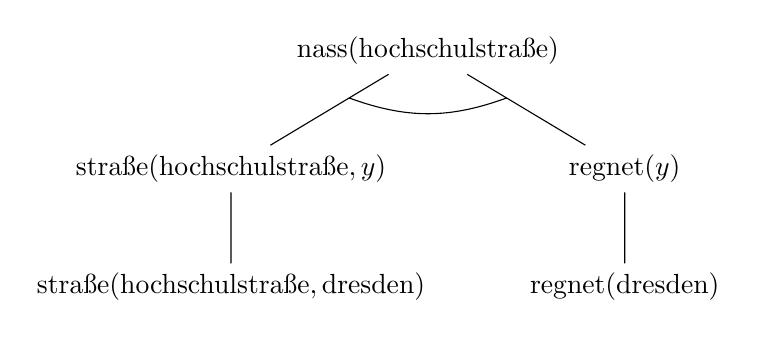
\begin{tikzpicture} 
\tikzstyle{level 1} = [sibling distance = 50 mm]
\tikzstyle{level 2} = [sibling distance = 30 mm]
\node(a){$\text{nass}(\text{hochschulstraße})$}
    child{node(b){$\text{straße}(\text{hochschulstraße},y)$}%TODO 2015-03-30T12:03
        child{node{$\text{straße}(\text{hochschulstraße},\text{dresden})$}}
        }
    child{node(d){$\text{regnet}(y)$}
        child{node{$\text{regnet}(\text{dresden})$}}
        }
    ;
\draw($(a)!0.4!(b)$) to[bend right=20]($(a)!0.4!(d)$);
\end{tikzpicture}\\

\paragraph{Definition}
Zwei Atome $P,Q$ heißen \underline{unifizierbar}, wenn es eine Ersetzung der in $P,Q$ verkommenden Variablen gibt, so dass $P \equiv Q$.

\subparagraph{Beispiel} $\text{regnet}(y),\text{regnet}(\text{dresden})$ sind unifizierbar durch $y / \text{dresden}.$\\ $P(a,X,Y),P(a,b,c)$ sind unifizierbar durch $X/b,Y/c.$\\ $P(X,X),P(a,b)$ sind nicht unifizierbar.

\subsubsection{Durchsuchen des Baums} Für ein Ziel $P$ wird das Prolog-Programm von oben nach unten durchsucht, bis eine linke Seite einer Klausel(Kopf) mit $P$ unifiziert. Dadurch wird ein neues Ziel erzeugt. Wenn dieses neue Ziel false liefert, wird ein Backtracking ausgeführt, indem eine weitere linke Seite gesucht wird, die mit dem Ziel unifiziert. Innerhalb jeder Klausel wird die rechte Seite von links nach rechts durchsucht.
\paragraph{Problem bei der Tiefensuche}
Beispiel: 
\begin{lstlisting}[numbers=left, tabsize=4, language=Prolog]
zug(X,Y) :- zug(Y,X).
zug(1,2).
?- zug(2,1).
\end{lstlisting}
Suchbaum\\
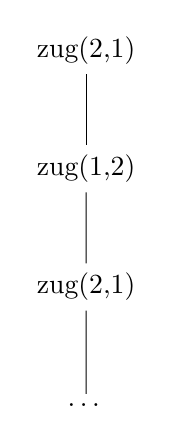
\begin{tikzpicture} 
\tikzstyle{level 1} = [sibling distance = 50 mm]
\tikzstyle{level 2} = [sibling distance = 30 mm]
\node{zug(2,1)}
        child{node{zug(1,2)}
            child{node{zug(2,1)}
                child{node{\dots}}
            }
        }
    ;
\end{tikzpicture}\\
Da der Suchbaum unendlich ist, liefert die Tiefensuche keine Lösung.

Lösung: Klauseln anders anordnen: Abbruchbedingung der Rekursion nach oben:
\begin{lstlisting}[numbers=left, tabsize=4, language=Prolog]
zug(1,2).
zug(X,Y) :- zug(Y,X)
\end{lstlisting}

Die Auswertestrategie von oben nach unten lässt sich nutzen, um ein if-else zu implementieren.
\begin{lstlisting}[numbers=left, tabsize=4, language=Prolog]
strasse(regen,nass).
strasse(X,trocken) :- X \== regen.
?-strasse(sonne,Y).
y=trocken.
\end{lstlisting}

\section{Computeralgebra}
\subsection{Arithmetik in Prolog}
Arithmetische Ausdrücke werden mit dem Operator "`is"' ausgewertet. Dabei muss die rechte Seite instanztiiert sein. Beispiel
\begin{lstlisting}[numbers=left, tabsize=4, language=Prolog]
?- X is 3+4.
X=7.
? 10 is 1+2.
false.
? 2 is 1+X.
Error.
\end{lstlisting}
\subparagraph{Beispiel} Berechnung von $n!$
\begin{lstlisting}[numbers=left, tabsize=4, language=Prolog]
fac(0,1).
fac(N,M) :- N1 is N-1,
            fac(N1,F),
            M is N * F.
\end{lstlisting}
\begin{tabular}{c|c|c}
Vergleichsoperatoren & Bedeutung & Beispiel\\ \hline
$==$ & identisch & $p(X) == p(X)$\\
$\backslash ==$ & nicht identisch & $p(X) \backslash == p(Y)$ \\
$=$ & unifizierbar & $p(X) = p(Y)$ \\
$\backslash = $ & nicht unifizierbar & $p(X) \backslash = q(X)$\\
$=:=$ & arithmetisch gleich & $2 =:= 1+1$\\
$= \backslash =$ & arithmetisch ungleich & $3 = \backslash = 1+1$\\
\end{tabular}\\
Prolog ist in der Lage, mit Hilfe des Unifikationsoperators arithmetische Ausdrücke zu zerlegen, wobei die Priorität der Operatoren beachtet wird.
\begin{lstlisting}[numbers=left, tabsize=4, language=Prolog]
? - x + 3 * y = A+B.
A=x, B=3*y.
? x+y+z = A+B.
A= x+y, B = z.
\end{lstlisting}
\paragraph{Anwendung} Symbolisches Differenzieren \[\frac{dx}{dx} = 1 \wedge \frac{c}{dx} = 0 \wedge \frac{dx \cdot c}{dx} = \frac{dx}{dx} \cdot c \wedge \frac{d(f\pm g)}{dx} = \frac{df}{dx} \pm \frac{dg}{dx}\]
\begin{lstlisting}[numbers=left, tabsize=4, language=Prolog]
diff(X,X,1).
diff(C,X,0) :- atomic(C), C \== X.
diff(-F,X,-DF) :- diff(F,X,DF).
diff(C*F,X,C*DF) :- diff(C,X,0), diff(F,X,DF).
diff(F+G,X,DF+DG) :- diff(F,X,DF), diff(G,X,DG).
diff(F-G,X,DF-DG) :- diff(F,X,DF), diff(G,X,DG).
\end{lstlisting}
Wie lassen sich Terme wie $1*x+0$ vereinfachen?\\*
Ansatz: Prädikat $s/2$
\begin{lstlisting}[numbers=left, tabsize=4, language=Prolog]
s(0+A,A).
s(A+0,B) :- s(A,B).
s(1*A,A).
s(A*1,A).
s(A*0,0).
s(0*A,0).
s(A+B,C) :- number(A), number(B), C is A+B.
s(A-B,C) :- number(A), number(B), C is A-B.
s(A*B,C) :- number(A), number(B), C is A*B.
s(A/B,C) :- number(A), number(B), C is A/B.
s(A+B,C) :- s(A,SA),s(B,SB),s(SA+SB,C).
s(A,A).
\end{lstlisting}
Idee: Mit dem Prädikat $s/2$ werden die Terme rekursiv zerlegt, mit $s0/2$ werden elementare Vereinfachungen vorgenommen. Dadurch wird von oben nach unten ein Syntaxbaum aufgebaut und von unten nach oben vereinfacht.

\subsection{Listen}
Listen sind induktiv definiert:
\begin{itemize}
\item $[\; ]$ ist die leere Liste
\item Wenn $H$ ein Element und $T$ eine Liste sind, dann ist $[H|T]$ eine Liste, die aus $H$ und den Elementen in $T$ besteht.
\end{itemize}
Alternativ kann die Liste auch in der Form $[x_1,\dots,x_n]$ aufgeschrieben werden.
\subparagraph{Beispiel} für Listen: $[a,b,c], [a|[b,c]], [a,b,c,1,2,[u,v]]$
\subparagraph{Beispiel} für ein Prädikat auf einer Liste: $\text{member} /2$ z.B. 
\begin{lstlisting}[numbers=left, tabsize=4, language=Prolog]
member(X,[X|_]).
member(X,[_|T]) :- member(X,T).
\end{lstlisting}
Suchbaum für die Anfrage $\text{member}(b,[a,b,c,]).$:\\*
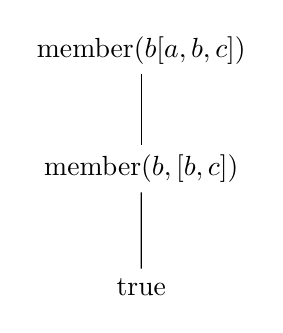
\begin{tikzpicture} 
\tikzstyle{level 1} = [sibling distance = 50 mm]
\tikzstyle{level 2} = [sibling distance = 30 mm]
\node{member$(b[a,b,c])$}
        %$X/b,T/[b,c]$
        child{node{member$(b,[b,c])$}%[b|[c]]
            child{node{true}}%X/b
        }
        
;
\end{tikzpicture}

Weiteres Listenprädikat: append$/$3\\
append$(L1,L2,L3)$ ist wahr genau dann, wenn die Verkettung der Listen $L1,L2$ gleich $L3$ ist.
\subparagraph{Beispiel} append$([a,b,c],[d,e,f],L)$ liefert $L=[a,b,c,d,e,f]$\\
append$([1,2,3],L,[1,2,3,4,5])$ liefert $L=[4,5]$\\
append$(L1,L2,[1,2,3])$ liefert $L1 = [], L2=[1,2,3]; L1=[1], L2=[2,3];$ usw.

\section{Sprachverarbeitung}
Beispielgrammatik:\\*
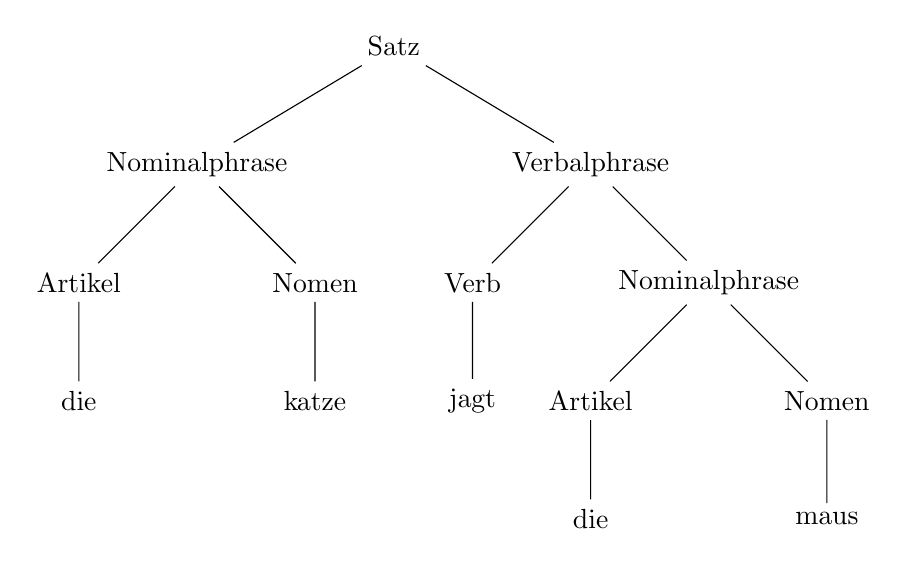
\begin{tikzpicture} 
\tikzstyle{level 1} = [sibling distance = 50 mm]
\tikzstyle{level 2} = [sibling distance = 30 mm]
\node{Satz}
        child{node{Nominalphrase}
            child{node{Artikel}
                child{node{die}}
            }
            child{node{Nomen}
                child{node{katze}}
            }
        }
        child{node{Verbalphrase}
            child{node{Verb}
                child{node{jagt}}
            }
            child{node{Nominalphrase}
                child{node{Artikel}
                    child{node{die}}
                }
                child{node{Nomen}
                    child{node{maus}}
                }
            }
        }
;
\end{tikzpicture}\\
Zur Darstellung von Strings verwenden wir Listen, z.B. $[$die,katze,schläft$]$.\\
Zur Darstellung der Grammatik verwenden wir einen Recursive-Descent-Parser.\\
\begin{lstlisting}[numbers=left, tabsize=4, language=Prolog]
satz(In,Rest) :-
    nominalphrase(In,R),
    verbalphrase(R,Rest).
nominalphrase(In,Rest) :- artikel(In,R), nomen(R,Rest).
verbalphrase(In,Rest) :- verb(In,R), nominalphrase(R,Rest).
artikel(In,Rest) :- match(die,In,Rest).
verb(In,Rest) :- 
    match(jagt,In,Rest).
nomen(In,Rest) :-
    match(katze,In,Rest);
    match(maus,In,Rest).
match(X,[X|Rest],Rest).
\end{lstlisting}
\subparagraph{Beispiel}
\begin{lstlisting}[numbers=left, tabsize=4, language=Prolog]
match(katze,[katze,schlaeft],R).
? R= schlaeft.
match(katze,[maus],R).
? false.
\end{lstlisting}
\subparagraph{Beispiel} Suchbaum für die Anfrage nominalphrase$([\text{die},\text{katze}],[\;])$\\
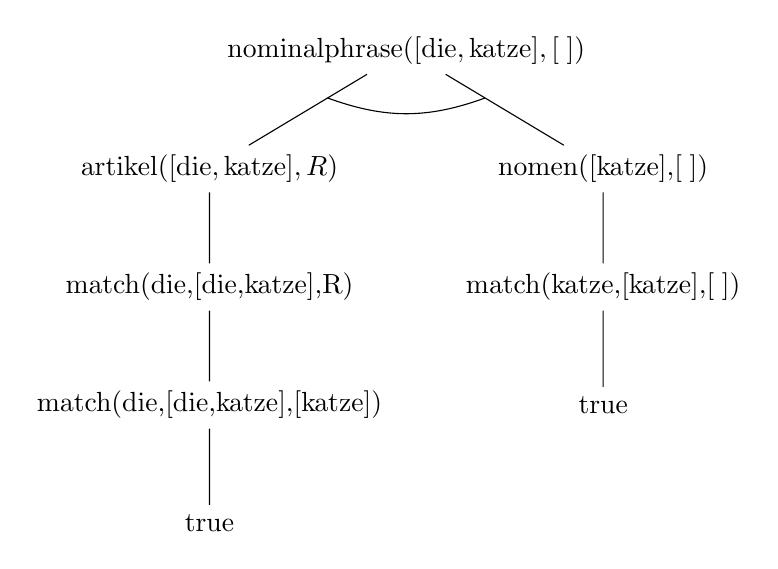
\begin{tikzpicture} 
\tikzstyle{level 1} = [sibling distance = 50 mm]
\tikzstyle{level 2} = [sibling distance = 30 mm]
\node(a){nominalphrase$([\text{die},\text{katze}],[\;])$}
    child{node(b){artikel$([\text{die},\text{katze}],R)$} %In/[die,katze], R/[]
        child{node{match(die,$[$die,katze$]$,R)}
            child{node{match(die,$[$die,katze$]$,$[$katze$]$)}
                child{node{true}}
            }
        }
    }
    child{node(d){nomen($[$katze$]$,$[\;]$)}
        child{node{match(katze,$[$katze$]$,$[\;]$)}
            child{node{true}}
        }
    }

;
\draw($(a)!0.4!(b)$) to[bend right=20]($(a)!0.4!(d)$);
\end{tikzpicture}
\paragraph{Genus-Kongruenz} Wenn das Nomen "`kater"' und der Artikel "`der"' in obige Grammatik eingefügt werden, können auch grammatikalisch falsche Sätze, wie $[$die,kater,jagt,der,maus$]$ abgeleitet werden.
\begin{lstlisting}[numbers=left, tabsize=4, language=Prolog]
nominalphrase(In,Rest) :- artikel(In,R,Genus), nomen(R,Rest,Genus).
artikel(In,Rest,m) :- match(der,In,Rest).
artikel(In,Rest,f) :- match(die,In,Rest).
nomen(In,Rest,m) :- match(kater,In,Rest).
nomen(In,Rest,f) :- 
    match(katze,In,Rest);
    match(maus,In,Rest).
\end{lstlisting}
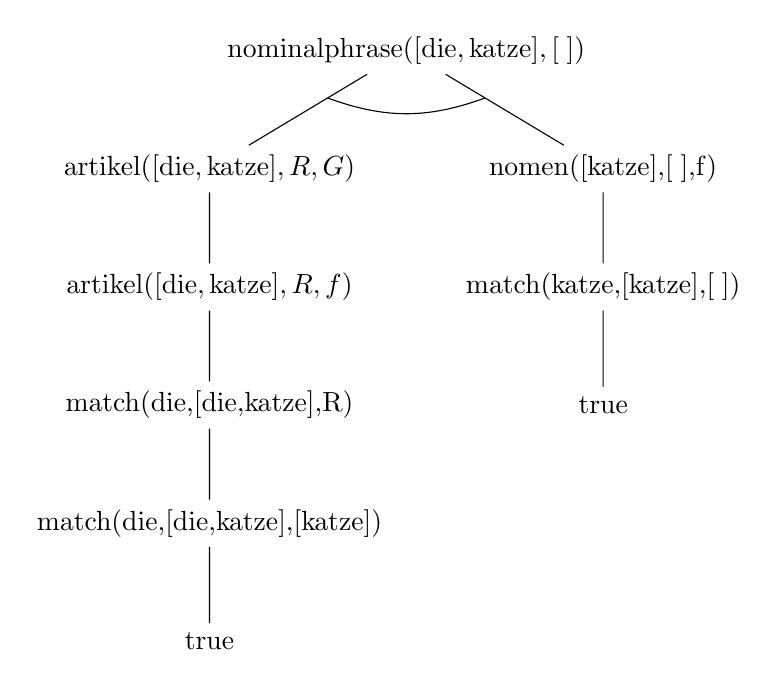
\begin{tikzpicture} 
\tikzstyle{level 1} = [sibling distance = 50 mm]
\tikzstyle{level 2} = [sibling distance = 30 mm]
\node(a){nominalphrase$([\text{die},\text{katze}],[\;])$}
    child{node(b){artikel$([\text{die},\text{katze}],R,G)$} %In/[die,katze], R/[]
        child{node{artikel$([\text{die},\text{katze}],R,f)$}
            child{node{match(die,$[$die,katze$]$,R)}
                child{node{match(die,$[$die,katze$]$,$[$katze$]$)}
                    child{node{true}}
                }
            }
        }
    }
    child{node(d){nomen($[$katze$]$,$[\;]$,f)}
        child{node{match(katze,$[$katze$]$,$[\;]$)}
            child{node{true}}
        }
    }

;
\draw($(a)!0.4!(b)$) to[bend right=20]($(a)!0.4!(d)$);
\end{tikzpicture}

\subsection{Wertigkeit von Verben}
Zwei wichtige Klassen von Verben sind:
\begin{itemize}
\item intransitive Verben: Diese zeihen kein Objekt nach sich (z.B. laufen, schlafen)
\item transitive Verben: Diese benötigen ein Objekt (z.B. sehen, fangen).
\end{itemize}
Das Verb bestimmt den Kasus des zugehörigen Objekts. Zum Beispiel benötigen jagen, fangen ein Akkusativobjekt (das Subjekt sieht wen oder was?)
\subsection{Dialogsystem}
Drei wichtige Aufgaben eines Dialogsystems
\begin{itemize}
\item Frage des Benutzers analysieren und den Sinn verstehen
\item Eine Antwort suchen
\item Antwort konstruieren und dem Benutzer antworten.
\end{itemize}
Einfacher Ansatz, um die Frage des Benutzers zu verstehen: Grammatik für mögliche Fragen des Benutzers konstruieren, die Parameter für die relevanten Bestandteile der Frage enthält. Anwendbar für einfach und gleichartig strukturierte Fragen, z.B. nach Zugverbindungen.
Aus der analysierten Frage erzeugt das Dialogsystem eine interne Repräsentation und durchsucht eine Wissensbasis und erzeugt daraus die Antwort.
\[ \text{place-question} \rightarrow (\text{in} | \varepsilon ) (\text{what} | \text{which} ) \text{Place 1 is the Place 2} (\text{on} | \text{in} | \text{located in} | \varepsilon ) \]
\[ \text{place 1} \rightarrow \text{street} | \text{town} | \text{city} \]
\[ \text{place 2} \rightarrow \text{hotel} | \text{restaurant} | \text{shop} \]

\section{Problemlösen durch Suche}
Viele Probleme der KI lassen sich auf eine systematische Suche in einem Wurzelbaum reduzieren.\\
Problem: Riesige Anzahl von Knoten in typischen Suchbäumen.
\subparagraph{Beispiel} Schach: Ca 30 Möglichkeiten pro Halbzug. Bei 50 Halbzügen enthält der Suchbaum $\sum\limits_{d=0}^{50} 30^d = \frac{30^{51}-1}{30-1} \approx 7,4 \cdot 10^{73}$ Knoten.\\
Bei 10000 Computern, die $10^9$ Knoten $s^{-1}$ erzeugen und durchsuchen können, ergibt sich für die Rechenzeit $2,3 \cdot 10^{53}$ Jahre.

\subsection{Uninformierte Suche}
Bereits bekannt: Breiten- und Tiefensuche\\
findall(X,P,L): sucht alle X, für die P wahr ist, und erzeugt daraus die Liste L.\\*
not(P): ist wahr genau dann, wenn P false liefert (Negation by failure).

\subsubsection{Nachteil der Breitensuche} Exponentieller Speicherbedarf für Suchbäume.
\subsubsection{Nachteil der Tiefensuche} 
\begin{itemize}
\item Wenn bereits besuchte Knoten nicht speichert werden: Zyklen möglich.

Lösung: In der Tiefensuche werden nur die Knoten auf dem aktuellen Pfad gespeichert. Der Platzbedarf liegt dann in $\mathcal{O}(d)$, wobei $d$ die Länge des aktuellen Pfades ist.

\item Der gefundene Weg ist nicht notwendig der kürzeste Weg.

\item Die Tiefensuche kann sich in unendlichen oder sehr langen Pfaden verlieren.

\end{itemize}

\subsection{Iterative Tiefensuche (IDDFS, Iterative Deepering Depth First Search)} 
Wir verwenden eine Tiefenschranke, die sukzessive erhöht wird, bis das Ziel gefunden wird.\\
Da in einem Suchbaum mit Verzweigungsfaktor $b>1$ fast alle Knoten Blätter sind, fällt die meiste Rechenzeit zum Durchsuchen der Blattebene an. Durch eine genaue Rechnung lässt sich zeigen, dass die Laufzeit der iterativen Tiefensuche nur einen kleinen Faktor höher ist, als die der Tiefensuche.

\subsection{Planungsprobleme}
\paragraph{Gegeben} Regeln, wie Zustände verändert werden können,
Startzustand und Zielzustand.
\paragraph{Gesucht} Weg vom Start zum Ziel.
\subparagraph{Beispiel} Affe-Banane-Problem: Gegen sei ein Raum mit einer Tür, einem Fenster, einem Affen und einer Banane. Im Ausgangszustand ist der Affe an der Tür, auf der gegenüber liegenden Seite ist das Fenster mit dem Stuhl in einer Ecke am Fenster und die Banane hängt in der Mitte des Raums von der Decke.\\
Problem: Der Affe ist nicht hoch genug um die Banane direkt zu greifen.\\
Regeln. Affe kann herumlaufen, den Stuhl verschieben, auf den Stuhl steigen.\\
Ziel: Affe auf dem Stuhl, unter der Banane.

Repräsentation eines Zustands, bzw. Knoten des Graphen:
\begin{itemize}
\item Position des Affen
\item Position des Stuhls
\item Position der Banane
\item Affe auf Stuhl
\end{itemize} [Anmerkung: Knoten repräsentieren somit den Gesamtzustand des Raumes]\\
Positionen: Tür, Mitte, Fenster.\\
Die Kanten des Graphen sind durch Regeln gegeben.

\subsection{Informierte bzw. heuristische Suche}
\paragraph{Ziel} Informationen über das Suchproblem nutzen, um schneller zum Ziel zu kommen. Dazu wird eine Bewertungsfunktion für die Knoten verwendet.\\
Die heuristische Suche verwendet eine heuristische Bewertungsfunktion \[ f: V \rightarrow \mathbb{R}_0^+ \]
Für den Zielknoten $v$ gilt : \[ f(v) = 0\] Die Knoten mit der niedrigsten Bewertung werden zuerst verfolgt.

\subsubsection{Gierige Suche}
Die gierige Suche verwendet in jedem Schritt den Knoten, der dem Ziel am nächsten liegt bzw., der die günstigste Entfernungsschätzung bis zum Ziel hat.
\subparagraph{Beispiel} Suche nach Wegen zu einem Ort.
Heuristische Bewertungsfunktion: $f(s) =$ Luftlinienentfernung von $s$ zum Ziel.\\
\begin{tikzpicture} 
\tikzstyle{level 1} = [sibling distance = 50 mm]
\tikzstyle{level 2} = [sibling distance = 30 mm]
\node{A}
    child{node(C){C}}
    child{node(B){B}};
    
\node{Z};
\end{tikzpicture}\\
Die kürzeste Strecke von A nach Z ist A-B-Z (100km). Wenn $f(C) < f(B)$, findet die gierige Suche jedoch die Strecke A-C-Z, die 11 km länger ist. 
\subparagraph{Folgerung} Die gierige Suche ist nicht optimal.

\subsection{$\text{A}^*$-Suche}
Die gierige Suche berücksichtigt nicht die Kosten, die bis zum Knoten $s$ bereits entstanden sind. Wir führen daher eine Funktion $g$ ein, die diese Kosten angibt, und eine Funktion $h$, die die Kosten bis zum Ziel schätzt.\\
Damit definieren wir die heuristische Bewertungsfunktion $f$ durch \[f(s) = g(s) + h(s)\]
Obige gierige Suche ist der Spezialfall $g(s) = 0, h(s) =$ Luftlinienentfernung bis zum Ziel.

\paragraph{Definition} Eine heuristische Kostenschätzfunktion $h$ heißt zulässig, wenn $h$ die Kosten bis zum Ziel nie überschätzt.\\
D.h. es gilt stets $h(s) \leq$ tatsächliche Entfernung von $s$ bis zum Ziel.

Die $\text{A}^*$-Suche ist folgender Algorithmus:\\*
Für den aktuellen Knoten $v$ werden die noch unbesuchten Nachbarn bestimmt und anhand ihrer heuristischen Bewertungsfunktion $f$, die wie oben konstruiert sein muss, in eine geeignete Datenstruktur eingefügt. In jedem Schritt wird die Suche mit einem Knoten mit minimaler Bewertung weitergeführt.

\paragraph{Naive Implementierung} Wie bei der Breitensuche werden die noch zu besuchenden Knoten in einer Liste gespeichert. Diese wird anhand der $f$-Werte der Knoten sortiert, so dass am Kopf der Liste Knoten mit minimaler Bewertung steht.

\paragraph{Effiziente Implementierung} Ein \emph{Min-Heap} ist ein Binärbaum mit der Eigenschaft: Jeder Knoten besitzt einen Wert, der $\leq$ der Werte seiner Nachfolger ist.

\subparagraph{Beispiel}
\begin{tikzpicture} 
\tikzstyle{level 1} = [sibling distance = 50 mm]
\tikzstyle{level 2} = [sibling distance = 30 mm]
\node{1}
    child{node{3}
        child{node{8}}
        child{node{6}}
        }
    child{node{5}
        child{node{7}}
    }

;
\end{tikzpicture}\\
Die Heap-Operationen
\begin{itemize}
\item Entfernen der Wurzel
\item Hinzufügen eines neuen Knotens
\end{itemize} benötigen die Laufzeit $\mathcal{O} (\log{(n)})$

Die $\text{A}^*$-Suche ist optimal, vorausgesetzt, die Kostenschätzfunktion $h$ ist zulässig.\\
Vorteil der $\text{A}^*$-Suche: Bei guter Heuristik wird das Ziel oft deutlich schneller gefunden als mit einer uninformierten Suche.\\
Nachteil: Wie bei der Breitensuche müssen im Worst-Case alle Knoten im Speicher gehalten werden.

\subsection{$\text{IDA}^*$-Suche}
\paragraph{Ziel} Vorteile der $A^*$-Suche mit denen der iterativen Tiefensuche kombinieren. Dazu führen wir eine Schranke für die heuristische Bewertungsfunktion $f$ ein und erhöhen diese schrittweise.

\paragraph{Anwendung} 8-Puzzle: %TODO 2015-06-01
Darstellung als Graph:
Knoten: Brettstellungen.
Kanten: geben an, wie durch Verschieben eines Plättchens eine neue Brettstellung erreicht werden kann.

Darstellung einer Brettstellung in Prolog:\\
Jede Zeile ist eine Liste aus drei Elementen, das Brett eine Liste aus drei Zeilen.

Geeignete Heuristiken für die Suche im 8-Puzzle:
\begin{enumerate}
\item Hamming-Distanz: Anzahl der Plättchen die falsch stehen. Diese Heuristik ist zulässig, weil mindestens so viele Verschiebungen notwendig sind, wie Plättchen falsch stehen.
\item Manhattan- oder Cityblock-Distanz: Anzahl Verschiebungen die nötig sind, um ein Plättchen auf direktem Weg zum Ziel zu schieben, summiert über alle Plättchen.\\
Diese Heuristik ist zulässig, da für jedes Plättchen mindestens diese Anzahl an Verschiebungen nötig ist.
\end{enumerate}














\end{document}